
\documentclass[letterpaper]{article}
\usepackage[letterpaper,margin=1.75in,noheadfoot]{geometry}
\usepackage{color, enumerate, sectsty}
\usepackage[normalem]{ulem}
\usepackage{amsmath}
\usepackage{graphicx}
\graphicspath{ {Figures/} }

\newcommand{\reporttitle}{Implementation of Perceptron Algorithm}
\newcommand{\name}{Shiva Bhusal}
\newcommand{\course}{CS 6200}

\usepackage[bookmarks, colorlinks, breaklinks,
pdftitle={\name - \reporttitle},pdfauthor={\name}, unicode]{hyperref}
\hypersetup{linkcolor=magneta,citecolor=magenta,filecolor=magenta,urlcolor=[named]{WildStrawberry}}

%%% Start of our document 

\begin{document}
\begin{center}{\huge \scshape \reporttitle}\end{center}
\begin{center}\vspace{0.2em} {\Large \name\\}
  {\course}\end{center}
  
%%% Let's add sections here. 
  
  \section{Introduction}
  Perceptron is the simplest form of neural networks. 

  \section {Experimental Results}
  \subsection {DataSet generation}
  Dataset was generated by using a simple algorithm by gradually increasing the value of x,y,z with reference to the center of the sphere. This simple algorithm makes sure that all the points lie within the sphere of radius 2. 30 such datasets are created and passed as a [4*30] dimensional array to the training method[x,y,z and expected output] The training method takes only first 15 datasets of the array and the classifier is trained. The rest of the datasets are used to test the accuracy of the classifier. 

  The attached screenshot shows the dataset generation result: 

  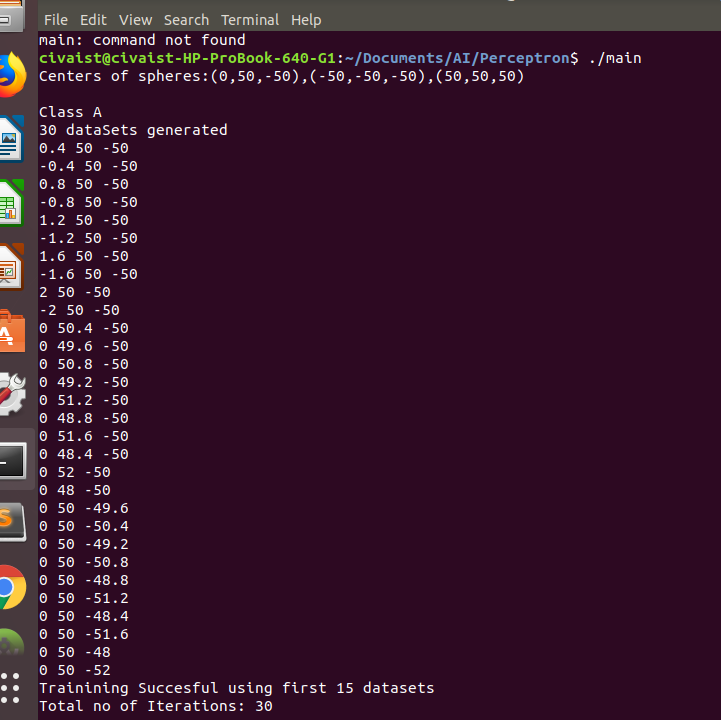
\includegraphics[width=8cm,height=8cm]{Dataset_generation}
  
  Similarly, datasets are also generated for the class B and Class C, and training is done seperately for each of the classes. 

  \subsection {Case 1: All the dataSets are linearly seperable}
  After the training was succesful, next 15 datasets were used for testing the classifier. The sample test result looked like this for the second half of the class A dataSets. Similar process was repeated for the second half of class B and class C datasets. 

  

  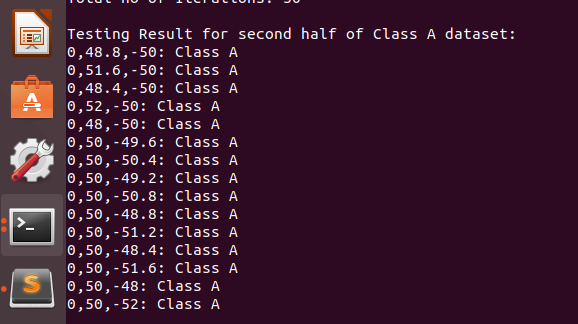
\includegraphics[width=10cm]{test_result}

  \subsection {Case 2: One of the Datasets is not linearly separable}

  \section {Summary}
  

\end{document}

%%% End of our document 
